\section{Polarization Cameras in the Maritime Domain}
Light behaves as a transverse wave, with its electromagnetic field oscillating in a plane perpendicular to the direction in which it travels.
With color filters the different frequencies of the ocsillation can be separated, and we can generate RGB images that make it easy to separate a red boat from a blue sea.
In a similar way, linear polarization filters can be used to separate light into its different polarization directions, which gives us a new set of tools to analyze the scene.


\subsection{Polarization Properties of Reflected Light}
When light is reflected off a surface, its polarization state changes \cite[34]{lingUniversityPhysicsVolume2016}.
This is illustrated in Figure \ref{fig:polarized_reflection} where the unpolarized light reflected off a surface becomes partially polarized.


\begin{figure}[H]
    \centering
    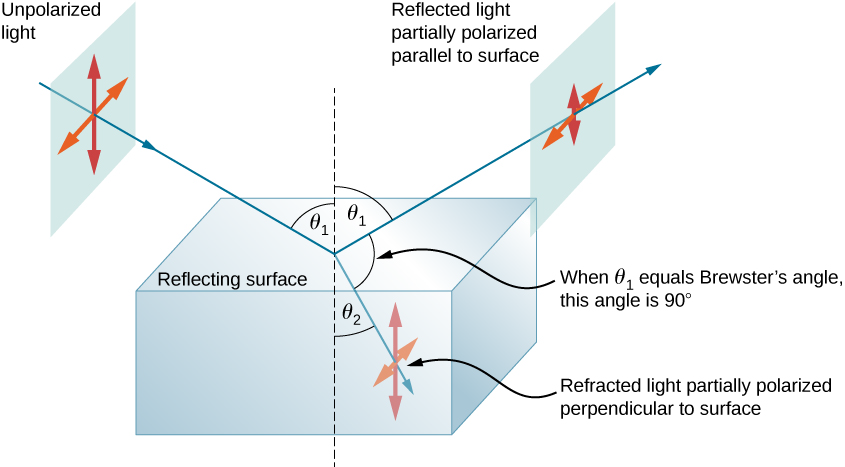
\includegraphics[width=.8\linewidth]{figures/polarization/reflaction.png}
    \caption{Polarization by reflection.
        \cite[Figure 1.38]{lingUniversityPhysicsVolume2016}}
    \label{fig:polarized_reflection}
\end{figure}


Unpolarized light can be described as a sum of two orthogonal linear polarizations $R_\perp$ and $R_\parallel$, where $R_\perp$ is perpendicular to the plane of incidence and $R_\parallel$ is parallel to the plane of incidence  \cite{FresnelEquations2024}.
These two components are referred to as s-polarized and p-polarized light, respectively.
Their reflection coefficients differ and are given by the Fresnel equations below \cite{FresnelEquations2024}:

\begin{align}
    R_\perp =         & \left|{\frac {n_{1}\cos \theta _1-n_{2}\cos \theta _2}{n_{1}\cos \theta _1+n_{2}\cos \theta _2}}\right|^{2}
                      &
    R_\parallel     = & \left|{\frac {n_{1}\cos \theta _2-n_{2}\cos \theta _1}{n_{1}\cos \theta _2+n_{2}\cos \theta _1}}\right|^{2}
\end{align}

Where  $\eta_1$ and $\eta_2$ are the refractive indices of the two media,
$\theta_i$ is the angle of incidence and $\theta_r$ is the angle of refraction.
Using the trigonometric identity $ \cos^2{\left(\theta_2 \right)} = 1- \sin^2{\left(\theta_2 \right)}$ and Snell's law $\eta_1 \sin{\left(\theta_1 \right)} = \eta_2 \sin{\left(\theta_2 \right)}$ the angle of refraction, $\theta_2$ can be removed, and the equations can be rewritten as:

\begin{align}
    R_\perp =         & \left|{\frac {n_{1}\cos \theta _1-n_{2}{\sqrt {1-\left({\frac {n_{1}}{n_{2}}}\sin \theta _1\right)^{2}}}}{n_{1}\cos \theta _1+n_{2}{\sqrt {1-\left({\frac {n_{1}}{n_{2}}}\sin \theta _1\right)^{2}}}}}\right|^{2}
                      &
    R_\parallel     = & \left|{\frac {n_{1}{\sqrt {1-\left({\frac {n_{1}}{n_{2}}}\sin \theta _1\right)^{2}}}-n_{2}\cos \theta _1}{n_{1}{\sqrt {1-\left({\frac {n_{1}}{n_{2}}}\sin \theta _1\right)^{2}}}+n_{2}\cos \theta _1}}\right|^{2}
\end{align}


Inserting the refractive index of air, $n_1 = 1$, and the refractive index of water, $n_2 = 1.33$, the reflectance can be calculated and plotted as a function of the angle of incidence, $\theta_1$, alone as shown in Figure \ref{fig:brewster0}.
The \gls{dolp} is the degree to which light is polarized and can be defined as the ratio between the difference and the sum of the two polarizations components.
The \gls{dolp} is plotted in Figure \ref{fig:brewster1}.
At one particular angle of incidence, $\theta_B$, known as the Brewser angle, $R_\parallel$ becomes zero, and the reflected light is completely s-polarized \cite{BrewsterAngle2024}:
\begin{align}
    \theta_B & = \arctan{\frac{n_2}{n_1}} & DoLP= & \frac{\left | R_\perp - R_\parallel \right |}{R_\perp + R_\parallel}
\end{align}

\begin{figure}[H]
    \centering
    \begin{subfigure}{.5\textwidth}
        \centering
        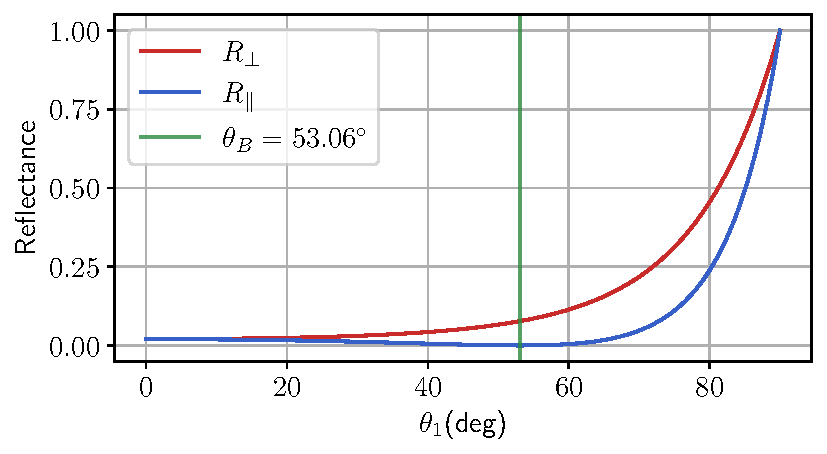
\includegraphics[width=\textwidth]{figures/pol_plots/brewster0.pdf}
        \caption{Reflectance of S and P polarized light of water.}
        \label{fig:brewster0}
    \end{subfigure}%
    \begin{subfigure}{.5\textwidth}
        \centering
        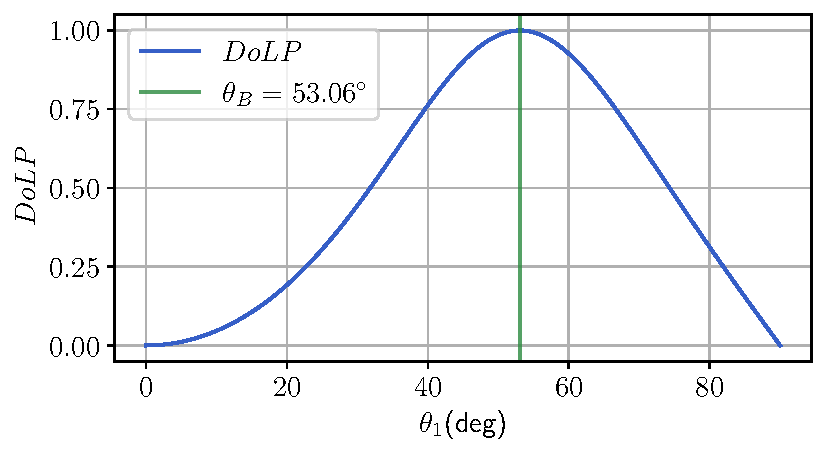
\includegraphics[width=\textwidth]{figures/pol_plots/brewster1.pdf}
        \caption{\gls{dolp} of light reflected off water.}
        \label{fig:brewster1}
    \end{subfigure}
    \caption{Reflectance and \gls{dolp} of light reflected off water as a funcion of of the angle of incidence.
        The Brewster angle is marked with a vertical line.}
    \label{fig:test}
\end{figure}




\subsection{Estimating Polarization Properties of Light using Polarizers}
In the case of polarized light, the electromagnetic oscillations trace an elliptical path, which simplifies to a circular or straight line for pure circular or linear polarization, respectively.
When light passes through a linear polarizer, the electric field is filtered, allowing only the component aligned with the polarizer to continue through.
By aligning four linear polarizers at 45-degree intervals, the \glsfirst{dolp} and \glsfirst{aolp} can be determined as shown in Figure \ref{fig:polarization_calculation}.

\begin{figure}[H]

    \begin{minipage}{.48\textwidth}
        % \begin{figure}[H]
        % \centering
        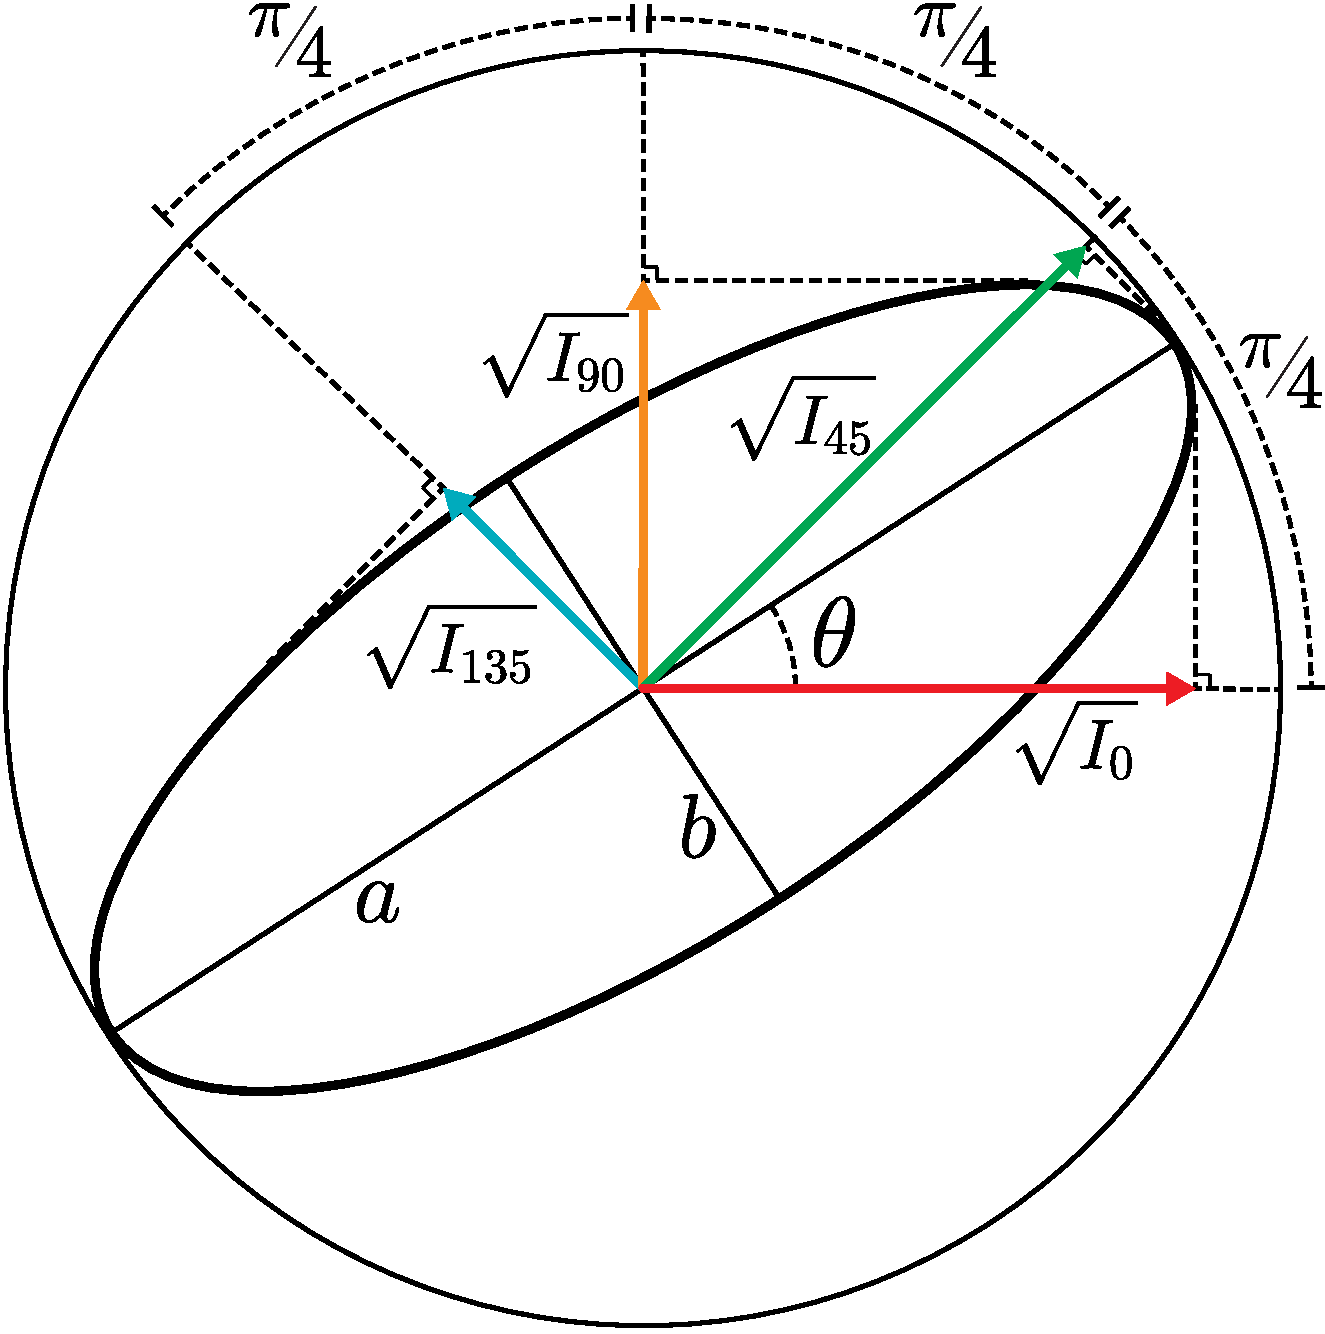
\includegraphics[width=\textwidth]{figures/polarization_sketch.pdf}
        % \label{fig:polarization_naming}
        % \end{figure} 
    \end{minipage}
    \hfill
    \begin{minipage}{.48\textwidth}
        \begin{alignat}{3}
             & \mathrlap{\cos\theta \cdot a\cos t -  \sin\theta \cdot b\sin t}                &
             &                                                                                &
             &                                                                                  \\
             &                                                                                &
             & = \mathrlap{\sqrt{a^2\cos^2\theta+b^2\sin^2\theta} \cos(\omega + \phi)}        &
             &                                                                                  \\[1em]
             & I_0                                                                            &
             & = \mathrlap{a^2\cos^2\theta + b^2\sin^2\theta                                } &
             &                                                                                  \\
             & I_{45}                                                                         &
             & = \mathrlap{a^2\cos^2(\theta-\frac{\pi}{4}) + b^2\sin^2(\theta-\frac{\pi}{4})} &
             &                                                                                  \\
             & I_{90}                                                                         &
             & = \mathrlap{a^2\sin^2\theta + b^2\cos^2\theta                                } &
             &                                                                                  \\
             & I_{135}                                                                        &
             & = \mathrlap{a^2\sin^2(\theta-\frac{\pi}{4}) + b^2\cos^2(\theta-\frac{\pi}{4})} &
             &                                                                                  \\[1em]
             & S_0                                                                            &
             & = I_0 + I_{90}                                                                 &
             & = a^2+b^2                                                                        \\
             & S_1                                                                            &
             & = I_0 - I_{90}                                                                 &
             & =(a^2-b^2)\cos(2x)                                                               \\
             & S_2                                                                            &
             & = I_{45} - I_{135}                                                             &
             & =(a^2-b^2)\sin(2x)                                                               \\[1em]
             & DoLP                                                                           &
             & =\frac{a^2-b^2}{a^2+b^2}                                                       &
             & = \frac{\sqrt{S_1^2 + S_2^2}}{S_0}                                               \\
             & AoLP                                                                           &
             & =  \theta                                                                      &
             & = \frac{1}{2}\arctan{\left(\frac{S_2}{S_1}\right)}
        \end{alignat}
    \end{minipage}%

    \caption{How four linear polarizers placed at $45^\circ$ intervals can be used to calculate the \gls{dolp} and \gls{aolp} of polarized light. The intensities  \label{fig:polarization_calculation}}
\end{figure}

\section{Polarization Cameras}
The sensor rig is equipped with two TRI050S1-QC cameras from Lucid Vision Labs.
The cameras are have a 5 MPixel \gls{cpfa} sensor, depicted in Figure \ref{fig:cpfa}, capabale of capturing both color and polarization information.

\begin{figure}[H]
    \begin{subfigure}[B]{.48\textwidth}
        \centering
        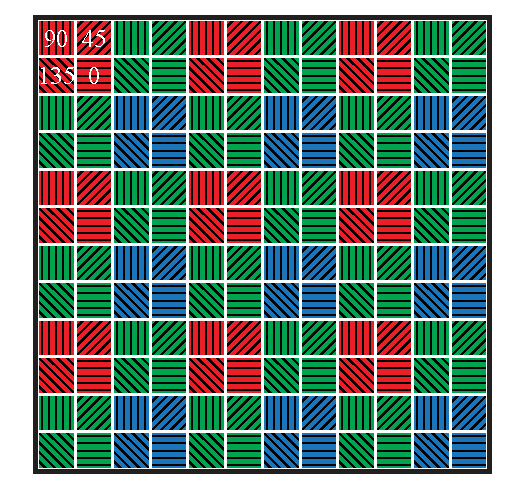
\includegraphics[width=\textwidth]{figures/sensor_layout.pdf}
        \caption{\gls{cpfa}. The numbers represents the filter angles.\label{fig:cpfa}}
    \end{subfigure}
    \hfill
    \begin{subfigure}[B]{.48\textwidth}
        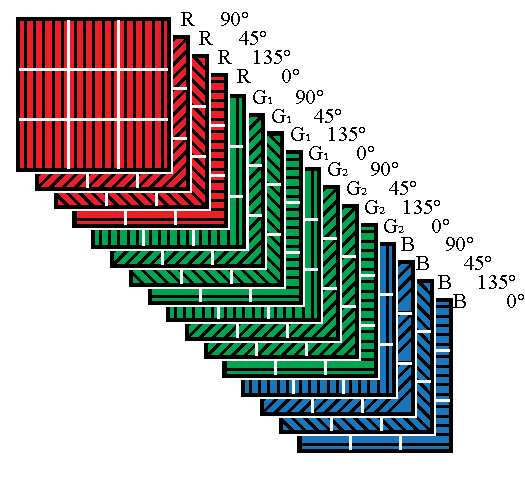
\includegraphics[width=\textwidth]{figures/sensor_packaging.pdf}
        \caption{Reordered view of \ref{fig:cpfa}. \label{fig:cpfa_reorder}}
    \end{subfigure}
    \caption{A 12\times12 slice of the \gls{cpfa} used in TRI050S1-QC cameras \cite{lucidvisionlabsTritonMPPolarized2020}, and how the the data can be reorderd as a 3\times3 image with 16 channels. \label{fig:polarization_sensor}}
\end{figure}

\subsection{Color-Polarization Demosaicking}
Similar to how demosacking is used to estimate the missing color channels in a Bayer filter array, the missing color and polarization information can be estimated from a \gls{cpfa} image.
We propose a new method where we estimate $S0$, $S1$, and $S2$ for each color channel at every pixel, resulting in a 9-channel image with the same resolution as the \gls{cpfa} image.

First the $n \times m \times 1$ input image is transformed to a $(n/4) \times (m/4) \times 16$ image, where the 16 channels correspond to the different color and polarization filters as depicted in Figure \ref{fig:polarization_sensor}.
This can be done by following these steps:
\begin{figure}[H]
    \centering
    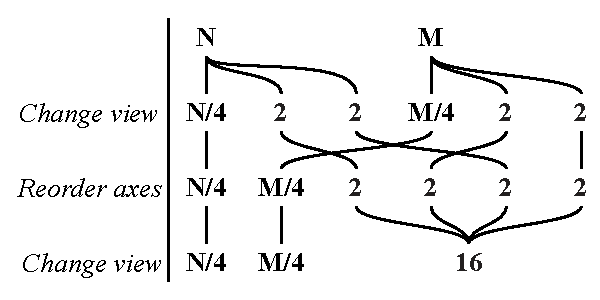
\includegraphics[width=.6\textwidth]{figures/transformation.pdf}
    % \caption{Steps performed to transform a $n \times m$ image with $c$ channels to a $n/4 \times m/4$ image with $16 \times C $ channels. This used to go from Figure \ref{fig:cpfa} to Figure \ref{fig:cpfa_reorder}. \label{fig:reorder_operations}}
\end{figure}%
With the goal of producing an $n \times m$ output image with 9 channels, we use a single $5 \times 5$ convolutional layer with $4*4*1=16$ input channels and $4*4*9=144$ output channels.
The output $n/4 \times m/4 \times 144$ channels can then be reored to a $n \times m \times 9$ image following a


With only $5\times5\times16\times144=57600$ parameters, it is possible to frame the optimization problem as an unconstrained quadratic problem and solve it directly on a RTX4090 GPU, without using any gradient descent based methods.
The Tokyo Tech dataset provides 40 12-channel images with 12 bit depth which we used to calculate the weights \cite{morimatsuMonochromeColorPolarization2020}.
Simulated camera data was generated by only picking the channel from each pixel with the same color and polarization angle as the corresponding pixel in a image from the TRI050S1-QC camera.
To increase the size of the dataset, we augmented it by shifting it up to 3 pixels in each direction to vary what

, and flipped them horizontally and vertically, effectively increasing the size of the dataset by a factor of $4\times4\times2\times2 =64$.
Similar results can


Wi fit the parameters in the convolution to the Tokyo Tech dataset \cite{morimatsuMonochromeColorPolarization2020}\cite{morimatsuMonochromeColorPolarization2021}, and augmented the data by shifting it up to 3 pixels in each direction and flipping it horizontally and vertically, effectively increasing the size of the dataset by a factor of $4\times4\times2\times2 =64$.
We noted that using 64 bit floating point numbers was necessary to avoid numerical instability.

Several methods already exists for performing color-polarization demosaicking on polarization cameras\cite{morimatsuMonochromeColorPolarization2020}\cite{morimatsuMonochromeColorPolarization2021}\cite{nguyenTwoStepColorPolarizationDemosaicking2022a}.





\begin{figure}[H]
    \begin{subfigure}[T]{.49\textwidth}
        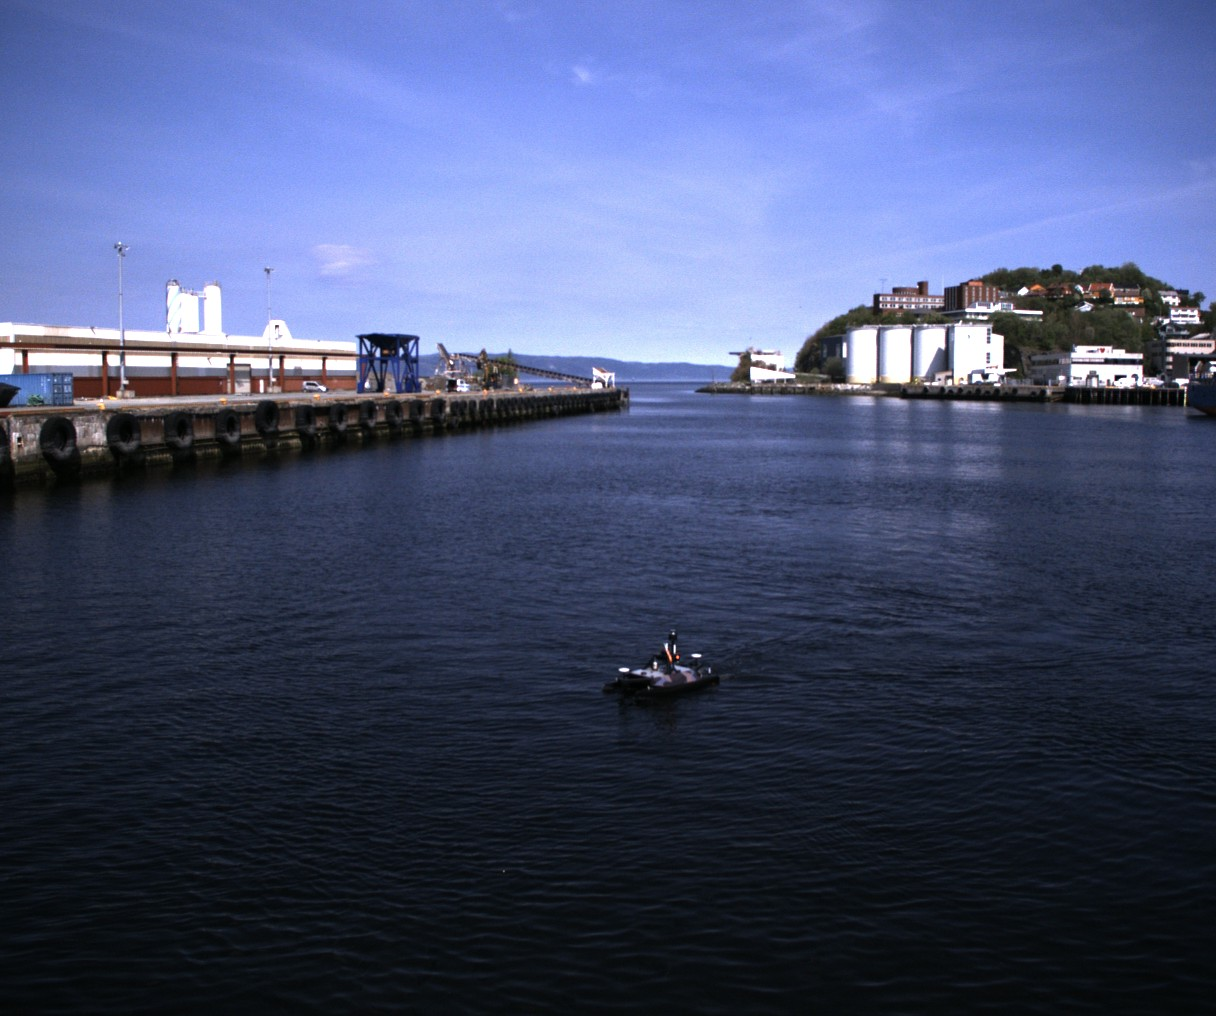
\includegraphics[width=\textwidth]{figures/img_0080_right_s0.jpg}
        \caption{S0, equivalent to what a normal camera would capture.}
    \end{subfigure}
    \hfill
    \begin{subfigure}[T]{.49\textwidth}
        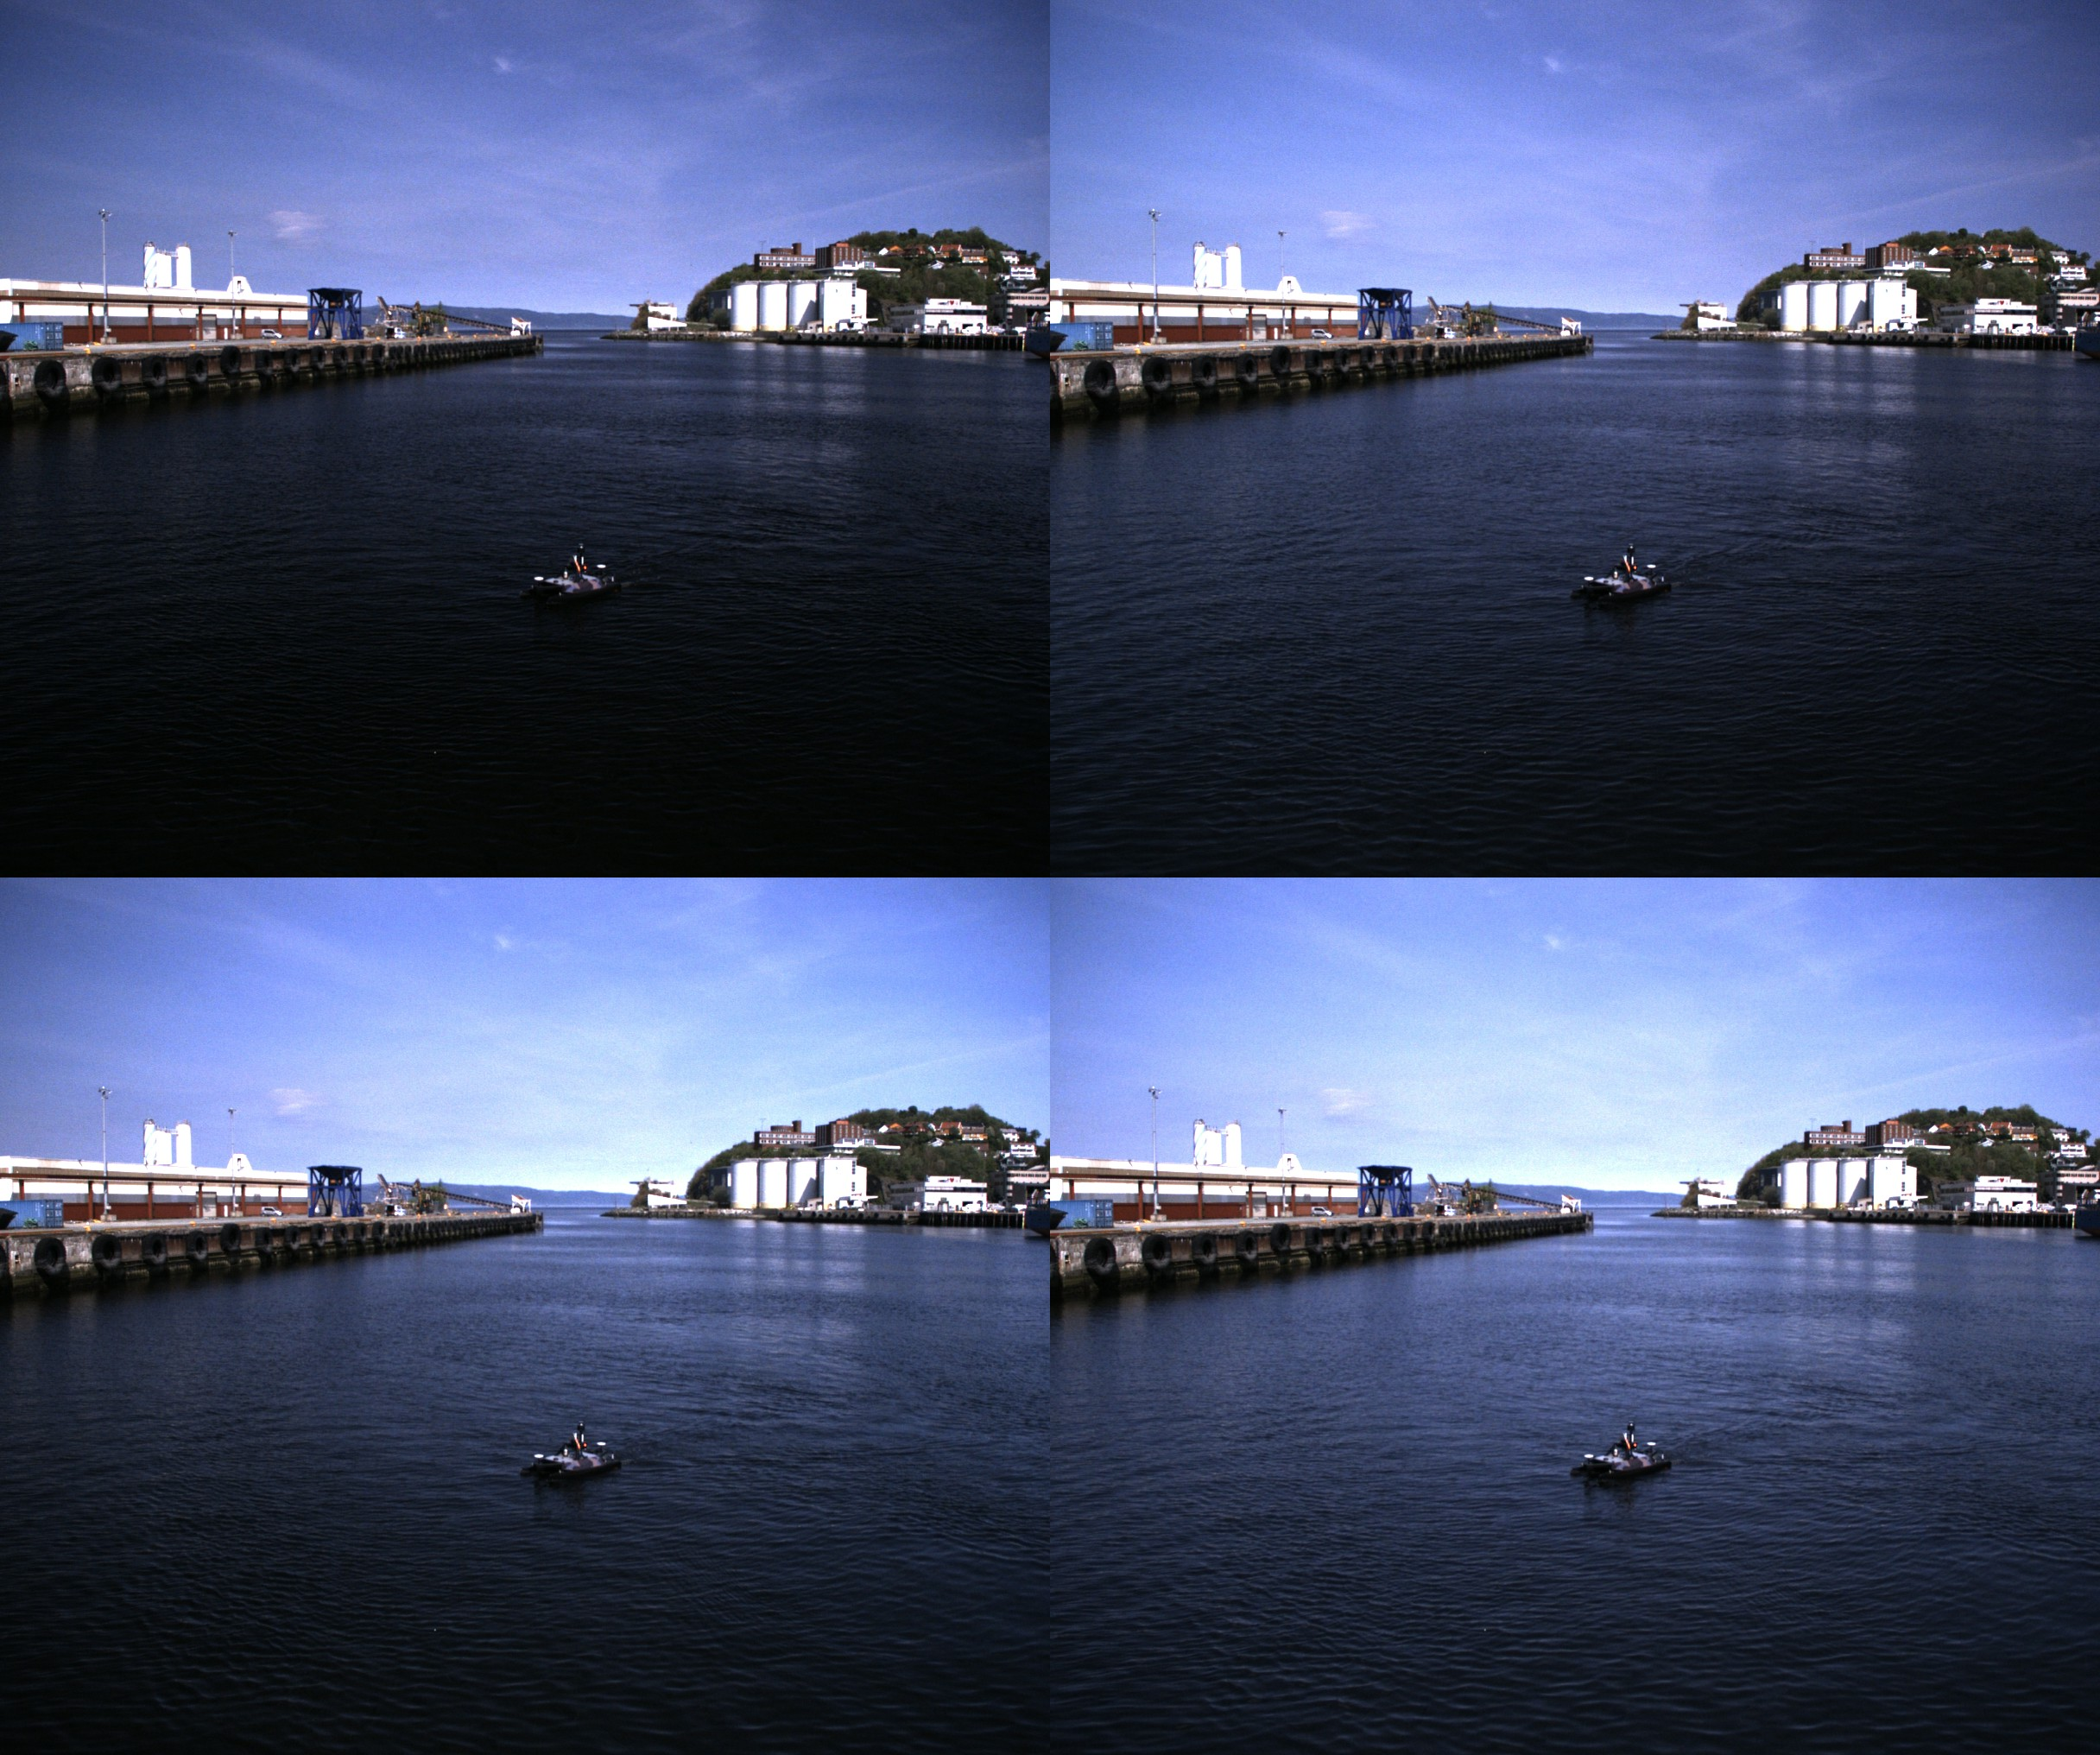
\includegraphics[width=\textwidth]{figures/img_0080_right_inten.jpg}
        \caption{I90, I45, I135, and I0.}
    \end{subfigure}

    \begin{subfigure}[B]{.49\textwidth}
        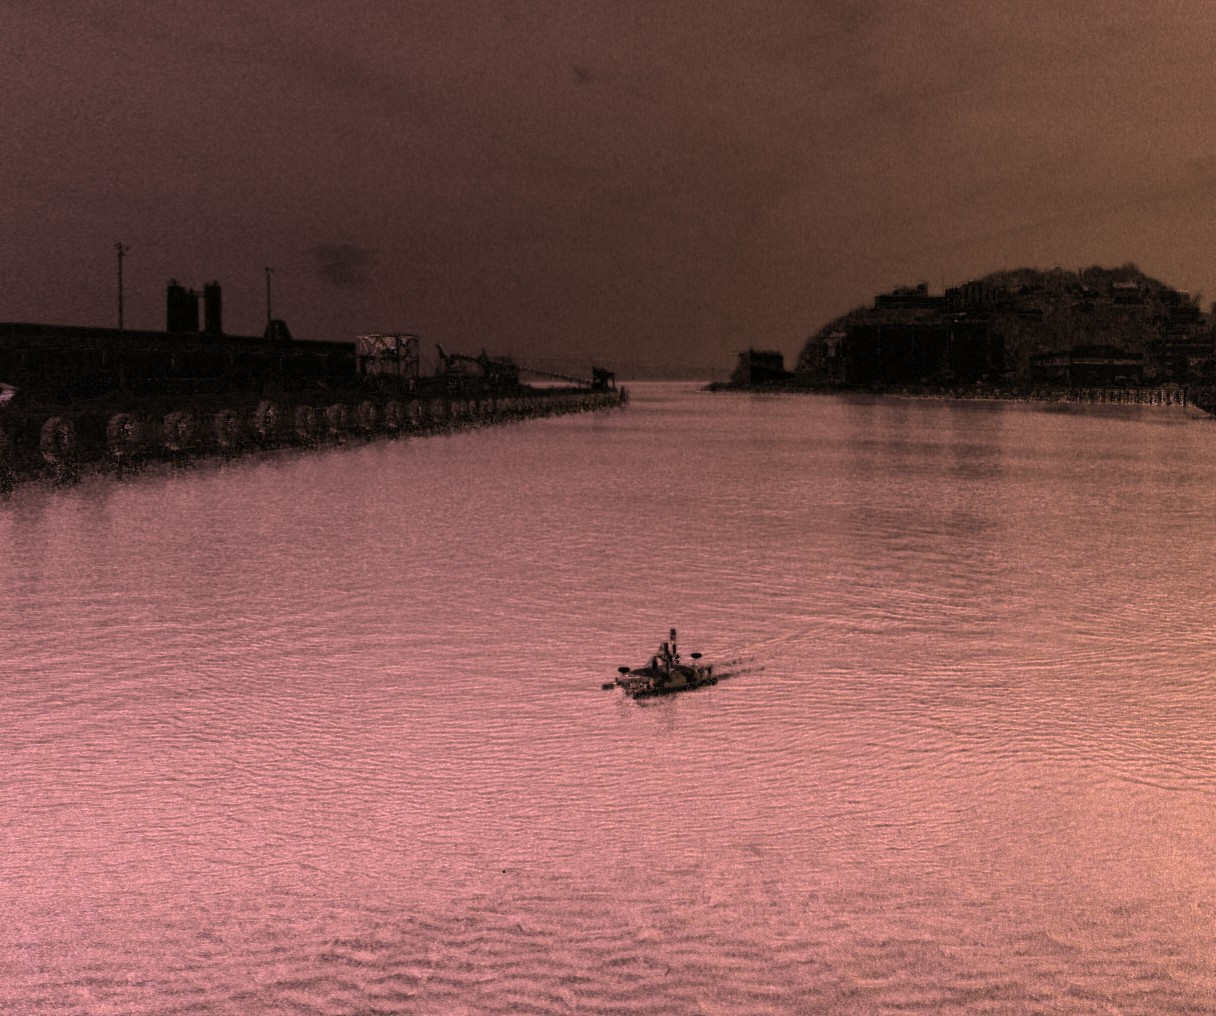
\includegraphics[width=\textwidth]{figures/img_0080_right_pol.jpg}
        \caption{Visualization of \gls{dolp} and \gls{aolp}}
    \end{subfigure}
    \hfill
    \begin{subfigure}[B]{.49\textwidth}
        \centering
        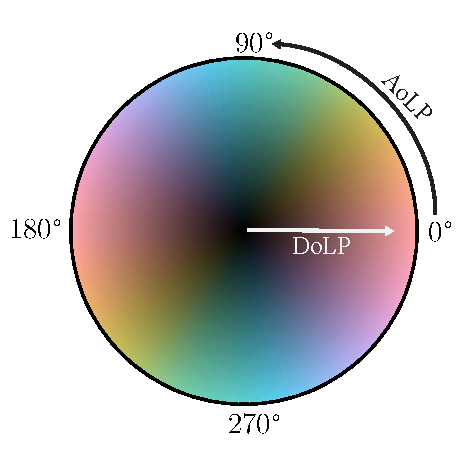
\includegraphics[width=.8\textwidth]{figures/cmap/aolp_dolp_cmap.pdf}
        \vspace{1em}
        \caption{Colormap}
    \end{subfigure}
    \caption{Visualization of an image captured with a color polarization filter array sensor. Note how the polarization information facilitates detection of the small vessel.}
\end{figure}
% \hfill

\subsection*{Color-Polarization Demosaicking}
Several methods already exists for performing color-polarization demosaicking \cite{morimatsuMonochromeColorPolarization2020}\cite{morimatsuMonochromeColorPolarization2021}\cite{nguyenTwoStepColorPolarizationDemosaicking2022a}.




In order to acheive high speed processing, we propose to formulate the debayering as a convolutional operation


There are other more advanced methods but a simple convolution works.
We propose to a general way to work with data from a color polarization filter array sensor.
As shown in Figure \ref{fig:cpfa_reorder}, an $n \times n$ raw image can be reordered as a $(n/4) \times (n/4) $ image with 16 channels.


% \section{Debayering of Color Polarization Images}

% \begin{align*}
%     \text{BT709} = \begin{bmatrix}
%                        0.2126  & 0.7152  & 0.0722  \\
%                        -0.1146 & -0.3854 & 0.5     \\
%                        0.5     & -0.4542 & -0.0458
%                    \end{bmatrix}
% \end{align*}


